%!TEX root = ../dokumentation.tex

\chapter{Theoretische Grundlagen}
\section{Elektromagnetische Wellen}
Als elektromagnetische Wellen werden sich räumlich ausbreitende Wellen bezeichnet, die aus elektrischen und magnetischen Feldern bestehen. Die laufende Welle breitet sich im Vakuum mit der Ausbreitungsgeschwindigkeit \(c\) von etwa \[c= 3*10^8 m/s\] aus. Die elektrischen und magnetischen Feldvektoren der Welle stehen orthogonal aufeinander, wie in Abbildung \ref{elektromagnetische Welle} gut zu erkennen ist.

\begin{figure}[ht]
	\centering
	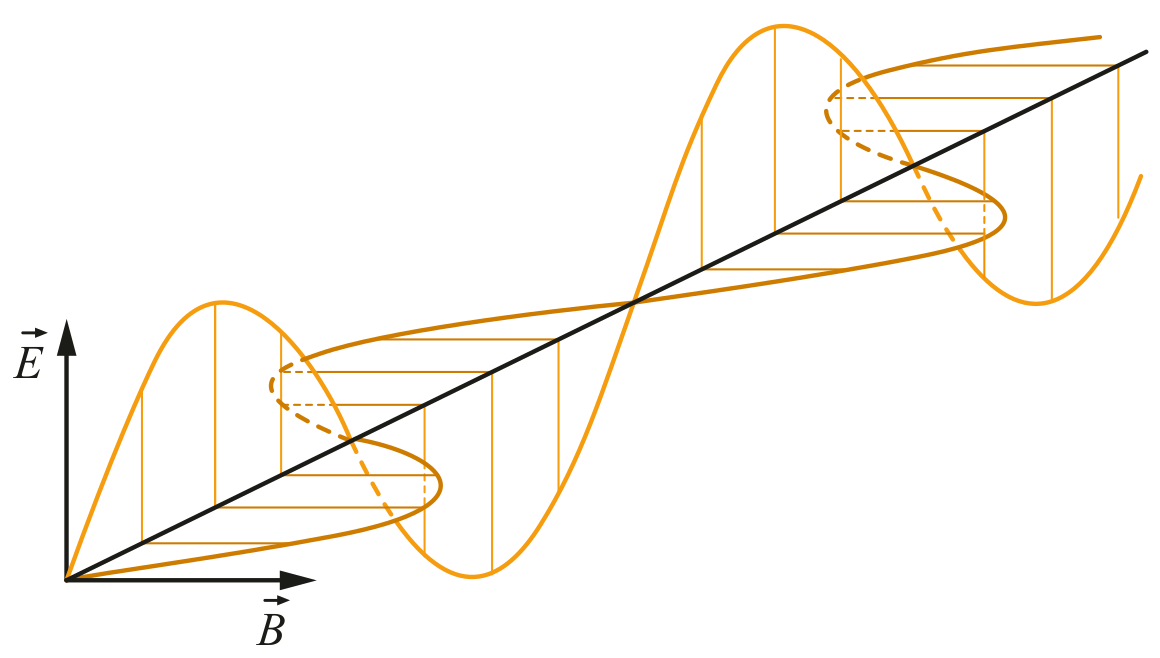
\includegraphics[width=0.75\textwidth]{em-welle.png}
	\caption[Elektromagnetische Welle mit senkrecht
	aufeinander stehendem elektrischem und magnetischem Feld]{Elektromagnetische Welle mit senkrecht aufeinander stehendem elektrischem und magnetischem Feld. Quelle: \cite[Harten, S. 130]{Harten:2017}} 
	\label{elektromagnetische Welle}
\end{figure}

Der Frequenzbereich, auch Spektrum genannt, solcher elektromagnetischen Wellen reicht von langsamen Radiowellen, Infrarotwellen über den Bereich des sichtbaren Lichts bis hin zur Röntgenstrahlung und der extrem kurzwelligen Gammastrahlung. In der Abschnitt \ref{section-frequenzbereiche} wird detaillierter auf die Frequenzbereiche eingegangen.

Die elektromagnetischen Wellen, welche auf die Erde einwirken werden auch als natürliche Strahlung bezeichnet.Elektromagnetische Wellen benötigen kein Medium, um sich auszubreiten. Sie können sich daher auch über weiteste Entfernungen ausbreiten. Sie bewegen sich im Vakuum unabhängig von ihrer Frequenz mit Lichtgeschwindigkeit fort. Elektromagnetische Wellen können sich aber auch in Materie ausbreiten wie etwa Gas oder Flüssigkeit, jedoch verringert sich dabei ihre Geschwindigkeit.

Die Existenz elektromagnetischer Wellen folgt aus den Maxwell-Gleichungen. Sie wurden 1886 von H. Hertz erstmals durch den elektrischen Schwingkreis erzeugt. Die Gleichungen werden im folgenden Kapitel genauer erklärt.

\section{Maxwellsche Gleichungen}

Die Maxwell-Gleichungen sind grundlegende Gleichungen der Elektrodynamik. Sie dienen zur Beschreibung der Phänomene des Elektromagnetismus und sie sind damit ein wichtiger Teil der Elektrodynamik. Mit Hilfe der Gleichungen können elektrische und magnetische Effekte beschrieben werden, etwa der Zusammenhang elektrischer und magnetischer Felder. Außerdem beschreiben sie die Korrelation elektrischer Ladungen und elektrischen Stroms durch definierte Randbedingungen. Maxwell beschrieb dadurch die Feldgrößen der elektrischen und magnetischen Felder und deren wirkenden Kräfte. 

\textbf{Maxwell-Gleichungen:}

Gaußscher Satz für Elektrizität		\[div \vec{E} = \frac{\rho}{\epsilon}\]		
Gaußscher Satz für Magnetismus 		\[div \vec{B} = 0\]
Faradaysches Gesetz					\[rot \vec{E} = -\frac{\partial\vec{B}}{\partial t}\]
Ampere-Maxwellsches Gesetz			\[rot \vec{B} = \mu\vec{j}+\epsilon\mu\frac{\partial\vec{E}}{\partial t}\]
\cite{halliday2017halliday}

Die dabei auftretenden Konstanten $\epsilon$ (elektrische Feldkonstante) und $\mu$ (magnetische Feldkonstante) sind im SI-Einheitensystem definiert. Die Abkürzungen div und rot stehen für Divergenz und Rotation. 

\subsection{Eigenschaften einer elektromagnetischen Welle}
Wie oben beschrieben besteht Licht aus elektrischen und magnetischen Feldern, die sich wellenförmig ausbreiten und somit eine elektromagnetische Welle darstellen. Beschrieben werden solche Wellen normalerweise als Sinussignal, welche durch Wellenlänge, Frequenz, Amplitude und Phase charakterisiert wird.
\begin{description}
	\item[Wellenlänge] Als Wellenlänge auch $\lambda$ (Lambda) genannt, versteht man den Abstand zweier Punkte mit gleicher Phase. Punkte die im zeitlichen Ablauf die gleiche Auslenkung (Amplitude) und die gleiche Bewegungsrichtung haben. Die Angabe der Wellenlänge erfolgt normalerweise in nm.
	\begin{figure}[ht]
		\centering
		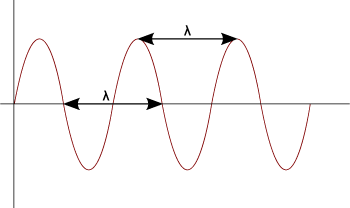
\includegraphics[width=0.5\textwidth]{wellenlaenge.png}
		\caption[Wellenlänge]{Wellenlänge. Quelle: \cite{uniwien:2018}}
		\label{Wellenlänge}
	\end{figure}
	\item[Amplitude] Die Amplitude oder auch Elongation $y$ genannt, beschreibt die maximale Auslenkung einer Schwingung.
		\begin{figure}[ht]
		\centering
		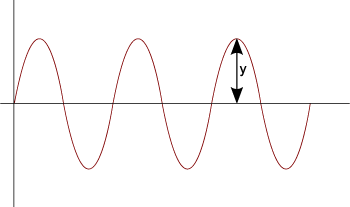
\includegraphics[width=0.5\textwidth]{amplitude.png}
		\caption[Amplitude]{Amplitude. Quelle: \cite{uniwien:2018}}
			\label{Amplitude}
		\end{figure}
	\item[Frequenz]Die Frequenz $f$ gibt die Anzahl der vollen Schwingungen  pro Zeiteinheit an und wird in Hertz (Hz = 1/s) angegeben.
	\item[Phase] Die Phase $\pi$ zeigt, an und zu welcher Position und Zeit die Minima und Maxima der Welle sich befinden.
\end{description}

\subsection{Elektronisches Rauschen}

Rauschen im Allgemeinen ist der Oberbegriff für Störspannungen, die ein Nutzsignal überlagern. Es wird als unerwünschtes Signal bezeichnet, das in Kommunikationssystem leider allgegenwärtig ist. Das Rauschen behindert den Empfang von Nachrichten bei der Übertragung, deshalb ist es erforderlich diesen Nebeneffekt zu begrenzen. Rauschen kann mehrere Ursachen haben, die alle durch physikalische Gesetzmäßigkeiten begründet werden können. Üblicherweise sind  Rauschen zufällig auftretende Störspannungen, die keine  Phasen oder Frequenzbeziehung zueinander haben. Dabei wird zwischen äußeren und inneren Rauschquellen unterscheiden.\newline

Rauschen im Allgemeinen ist der Oberbegriff für Störspannungen, die ein Nutzsignal überlagern. Es wird als unerwünschtes Signal bezeichnet, das in Kommunikationssystemen aber allgegenwärtig ist. Rauschen verhindert den Empfang von Nachrichten in ihrer ursprünglichen Form bei Übertragungen, deshalb ist es erforderlich diesen Nebeneffekt zu begrenzen. Rauschen kann mehrere Ursachen haben, die alle durch physikalische Gesetzmäßigkeiten begründet werden können. Üblicherweise wird Rauschen verursacht durch zufällig auftretende Störspannungen, die keine  Phasen oder Frequenzbeziehung zueinander haben.

äußere Rauschquellen: 
\begin{itemize}
	\item Hintergrundrauschen
	\item Kosmisches Rauschen
	\item Terrestrisches Rauschen
\end{itemize}
innere Rauschquellen:
\begin{itemize}
	\item Wärmerauschen
	\item Röhrenrauschen in Elektronenröhren
	\item 1/$f^2$-Rauschen
\end{itemize}

\newpage
\section{Nachrichten- und Übertragungstechnik}
Die Nachrichten- und Übertragungstechnik beschäftigt sich mit dem Übertragen elektronischer Nachrichten. Als Nachricht wird in diesem Kontext ein vom Sender gezielt erzeugtes Signal verstanden, welches mit Informationen behaftet und für den Empfänger der Nachricht bestimmt ist \cite[vgl. Werner, S. 3]{Werner:2006}.

Das in Abb. \ref{nachrichtenuebertragung} dargestellte Kommunikationsmodell nach Shannon beschreibt den Grundlegenden Aufbau eines Nachrichtenaustausches zweier Systeme. 
Im Folgenden werden die zum weiteren Verständnis notwendigen Begriffe eingeführt:\newline
Die Informationsquelle (\enquote{Information Source}) übergibt die Nachricht dem Sender (\enquote{Transmitter}), der diese mit einem Signal als physikalischem Träger der Nachricht über einen Kanal (\enquote{Channel}) sendet. \newline
Als Kanal bezeichnet man in der Nachrichtentechnik sämtliche technische Komponenten, welche eine Information vom Sender zum Empfänger transportiert. \cite[vgl. Dankmeier, S. 13]{Dankmeier:2017}.\newline
Die im Kanal auftretenden Störsignale, hier durch die Störsignalquelle (\enquote{Noise Source}) dargestellt, überlagern sich mit dem ursprünglichen Signal.\newline
Aus dem für den Empfänger (\enquote{Receiver}) bestimmten Empfangssignal (\enquote{Received Signal}) wird anschließend wieder eine Nachricht generiert, die im letzten Schritt der Informationssenke (\enquote{Destination}) übergeben wird.

\begin{figure}[ht]
	\centering
	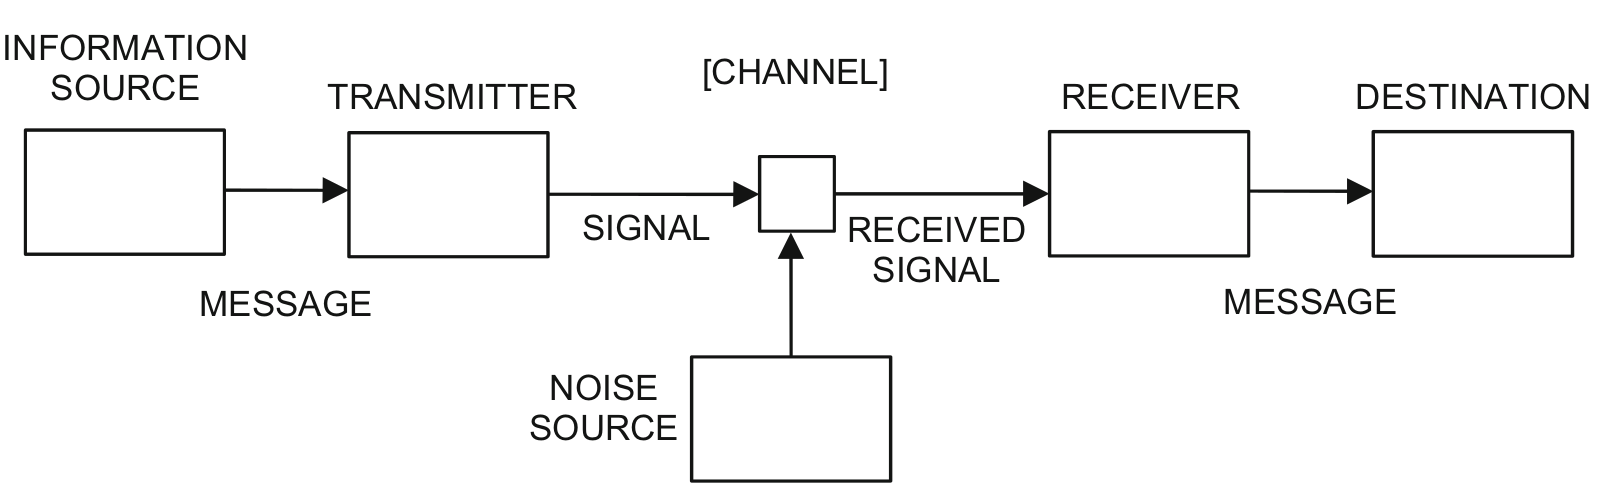
\includegraphics[width=\textwidth]{nachrichtenuebertragung-shannon.png}
	\caption[Kommunikationsmodell nach Shannon]{Kommunikationsmodell nach Shannon. Quelle: \cite[Werner, S. 11f]{Werner:2017}} 
	\label{nachrichtenuebertragung}
\end{figure}

Die von der Informationsquelle zu übertragenden Daten werden, je nach Datenquelle, durch eine Quellcodierung komprimiert und beim Empfänger dann durch die entsprechende Umkehroperation die ursprünglichen Daten wiederhergestellt.




\newpage
\section{Signale und Spektren}
Signale werden üblicherweise auf 2 Arten dargestellt:
\begin{enumerate}
	\item Als \textit{Signal} im Zeitbereich
	\item Als \textit{Spektrum} im Frequenzbereich
\end{enumerate}




\subsection{Kontinuierliche und diskrete Signale}
Als Signal gilt eine Funktion mit mindestens einer unabhängigen Variablen, beispielsweise der Zeit \(t\). Ist die Zeitvariable nur für diskrete Werte definiert, so spricht man von einem zeitdiskreten Signal. Man schreibt auch \(x[n]\), wobei \(n\) die normierte Laufvariable genannt wird \cite[vgl. Werner, S. 24]{Werner:2017}.

In Abb. \ref{kontinuierlich_diskret} wird das kontinuierliche Signal
\[x(t) = \sin \omega t = \sin 2\pi f t\]
mit \(f = 50 \text{ Hz} \) dargestellt und mit dem diskreten Signal
\[x[n] = x(nT_a) = \sin 2\pi f T_a n\]
überlagert, welches mit einer Abtastrate von \(f_a = 1 \text{ kHz}\) oder anders ausgedrückt: einem Abtastintervall von \(T_a = 1 / f_a = 1 \text{ ms}\) abgetastet wird \cite[vgl. Heuberger, e. a., S. 11f]{Heuberger:2017}. Das diskretisierte Signal wird also durch die Abtastpunkte repräsentiert und muss aus diesen rekonstruiert werden.

\begin{figure}[ht]
	\centering
	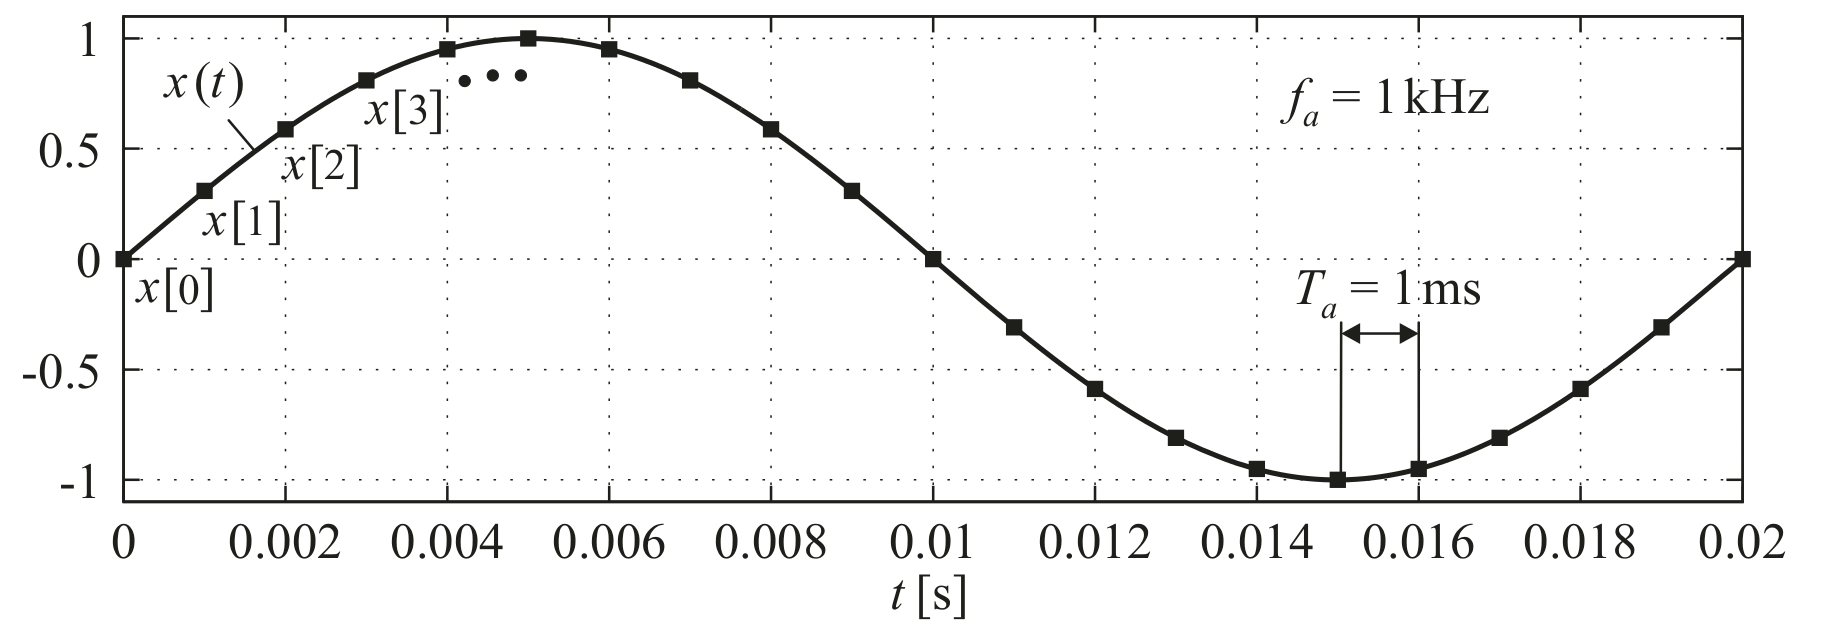
\includegraphics[width=\textwidth]{kontinuierlich-diskret.png}
	\caption[Sinusfunktion als kontinuierliches und als diskretes Signal]{Sinusfunktion als kontinuierliches und als diskretes Signal. \newline Quelle: \cite[Heuberger, e. a., S. 12]{Heuberger:2017}} 
	\label{kontinuierlich_diskret}
\end{figure}

%\subsection{Analoge und digitale Signale}
%Digitale Signale sind sowohl werte- als auch zeitdiskret.


\subsection{Nyquist-Shannon-Abtasttheorem}
Das Abtasttheorem nach Nyquist und Shannon besagt, dass ein Signal der Funktion \(x(t)\) welches die Frequenz \(f\) besitzt, mindestens mit der Abtastrate \(f_a\) abgetastet werden muss, wobei gilt: \(f_a \ge 2f\), damit aus dem abgetasteten Signal das Originale durch eine Interpolation ausreichend genau beschrieben werden kann \cite[vgl. Werner, S. 30]{Werner:2006}. 
Ist dies nicht der Fall, kann beim Abtasten zweier Signale unterschiedlicher Frequenzen dazu kommen, dass die resultierenden diskreten Signale identisch sind. Dieser Effekt wird als \enquote{Aliasing} bezeichnet:

\begin{figure}[ht]
	\centering
	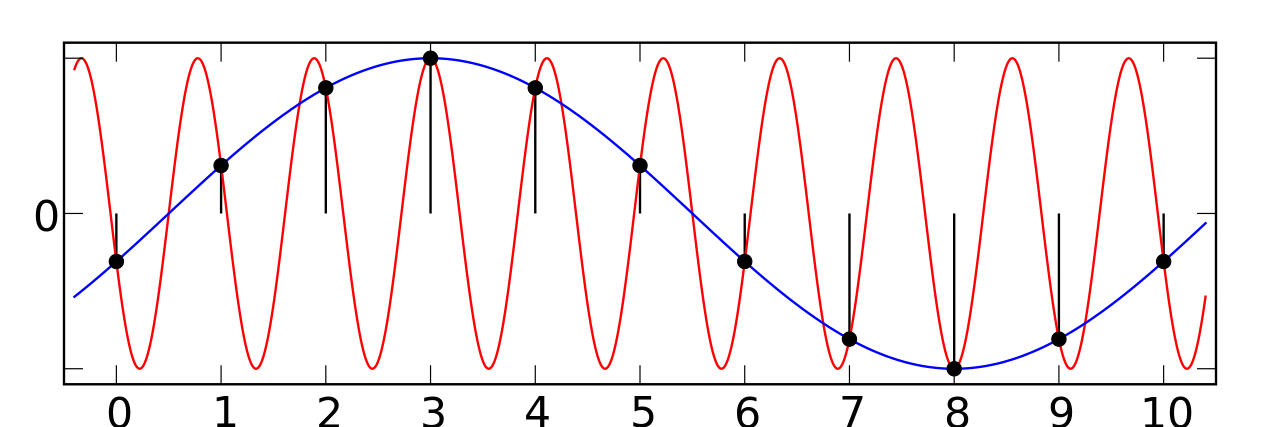
\includegraphics[width=0.9\textwidth]{aliasingsines.png}
	\caption[Aliasing Effekt. Abtastung zweier Sinussignale verschiedener Frequenzen]{Aliasing Effekt. Abtastung zweier Sinussignale verschiedener Frequenzen. \newline Quelle: \cite[Moxfyre]{aliasingsampling:2009}} 
	\label{abtasttheorem}
\end{figure}

Reale Signale bestehen meist jedoch nicht aus einer einzigen Frequenz. Sie haben verschiedene Frequenzanteile (zu denen auch das durch die Übertragung bedingte Rauschen gehört).
In der Praxis wird daher meist eine Abtastrate verwendet, die ausreichend größer ist, als der doppelte Betrag der höchsten Frequenzkomponente im gegebenen Signal.





\subsection{Spektrum eines Signals}
Eine alternative Darstellung von Signalen kann im Frequenzbereich erfolgen. Dort wir ein Signal mit mehreren Sinus-Schwingungen beschrieben, aus denen es sich zusammensetzen lässt \cite[vgl. Karrenberg, S. 42]{Karrenberg:2017}.





\subsection{Fourier-Transformation}
Um ein Signal aus dem Zeitbereich in den Frequenzbereich zu überführen wird die sogenannte Fourier-Transformation angewandt.\newline
Im wesentlichen wird ein Signal bzw. eine Funktion mittels Fourier-Transformation als Summe mehrerer Sinus-Schwingungen unterschiedlicher Frequenzen und Amplituden dargestellt.

Signale können also entweder aus Sinusschwingungen konstruiert, oder in solche zerlegt werden.
Nach der Zerlegung ergeben sich verschiedene Möglichkeiten mit den einzelnen Frequenzen zu arbeiten:
\begin{itemize}
	\item Aus einem Signal können einzelne Frequenzen hervorgehoben werden
	\item Bei Audiosignalen beispielsweise können ungewollte Frequenzen ausgeblendet werden (etwa Störgeräusche)
\end{itemize}

Um von dem resultierenden Spektrum wieder zu einer Darstellung im Zeitbereich zu gelangen, kann die Umkehroperation, die inverse Fourier-Transformation angewandt werden.

In der Praxis wird für die Überführung in den Frequenzbereich meist die \ac{FFT} genutzt \cite[vgl. Heuberger, e. a., S. 14]{Heuberger:2017}. Die \ac{FFT} ist allerdings nur eine effizientere Berechnungsart der \ac{DFT}, welche die Fouriertransformation auch mit diskreten Werten ermöglicht \cite[vgl. Meyer, S. 175]{Meyer:2017}.

Um ein Signal mittels \ac{FFT} in den Frequenzraum überführen zu können, muss es die Länge der Form \(N = 2^L\) aufweisen. \(N\) muss also eine 2er-Potenz sein \cite[vgl. Heuberger, e. a., S. 15]{Heuberger:2017}.
Für das zu überführende Signal gilt also:
\[\underline{x} = \Big[ \:  \underline{x}[0] \; \underline{x}[1] \; \underline{x}[2] \; ... \; \underline{x}[N - 2] \; \underline{x}[N - 1] \; \Big] \]





\subsubsection{Fensterfunktionen}
In der Praxis, so auch bei \ac{SDR}-Systemen, handelt es sich in der Regel um Ausschnitte eines Signales. Bei der \ac{FFT} wird mit periodischen Signalen gearbeitet, ein Signalausschnitt ist aber nur quasiperiodisch. Denn an den Rändern gibt es bei der periodischen Fortsetzung des Signals Sprungstellen \cite[vgl. Meyer, S. 187]{Meyer:2017}.\newline
Wird also ein Signal, dessen Länge kein vielfaches einer ganzen Periode ist, aufgezeichnet, entsteht durch die Unstetigkeiten am Rand eine spektrale Streuung durch die Umwandlung mit der \ac{FFT}.

Der Signalausschnitt wird deshalb mit einer sogenannten Fensterfunktion gewichtet: 
\[w = \Big[ \:  w[0] \; w[1] \; w[2] \; ... \; w[N - 2] \; w[N - 1] \; \Big] \]


Die gefensterte FFT Funktion:
\[\text{FFT} _w \: {\underline{x}[n]} = \sum_{n=0}^{N-1} w[n] \: \underline{x}[n] \: e^{-j2\pi nm / N} \text{ mit } m = 0, ..., N-1\]


Das Spektrum dieser Funktion lässt sich als den gewichteten Betrag des resultierenden Ergebnisses ausdrücken \cite[vgl. Heuberger, e. a., S. 14]{Heuberger:2017}:
\[s_x[m] = \frac{1}{c_w^2} \: \Big{|}\underline{X}[m]  \Big{|}^2 \text{ mit } c_w = \sum_{n=0}^{N-1} w[n] \]

In Abbildung \ref{fft} wird das diskrete Zeitsignal \(x[n]\) dem gefensterten Zeitsignal \(w[n]x[n]\) und dem aus der FFT resultierenden Spektrum \(S_x[m]\) gegenübergestellt:
\begin{figure}[ht]
	\centering
	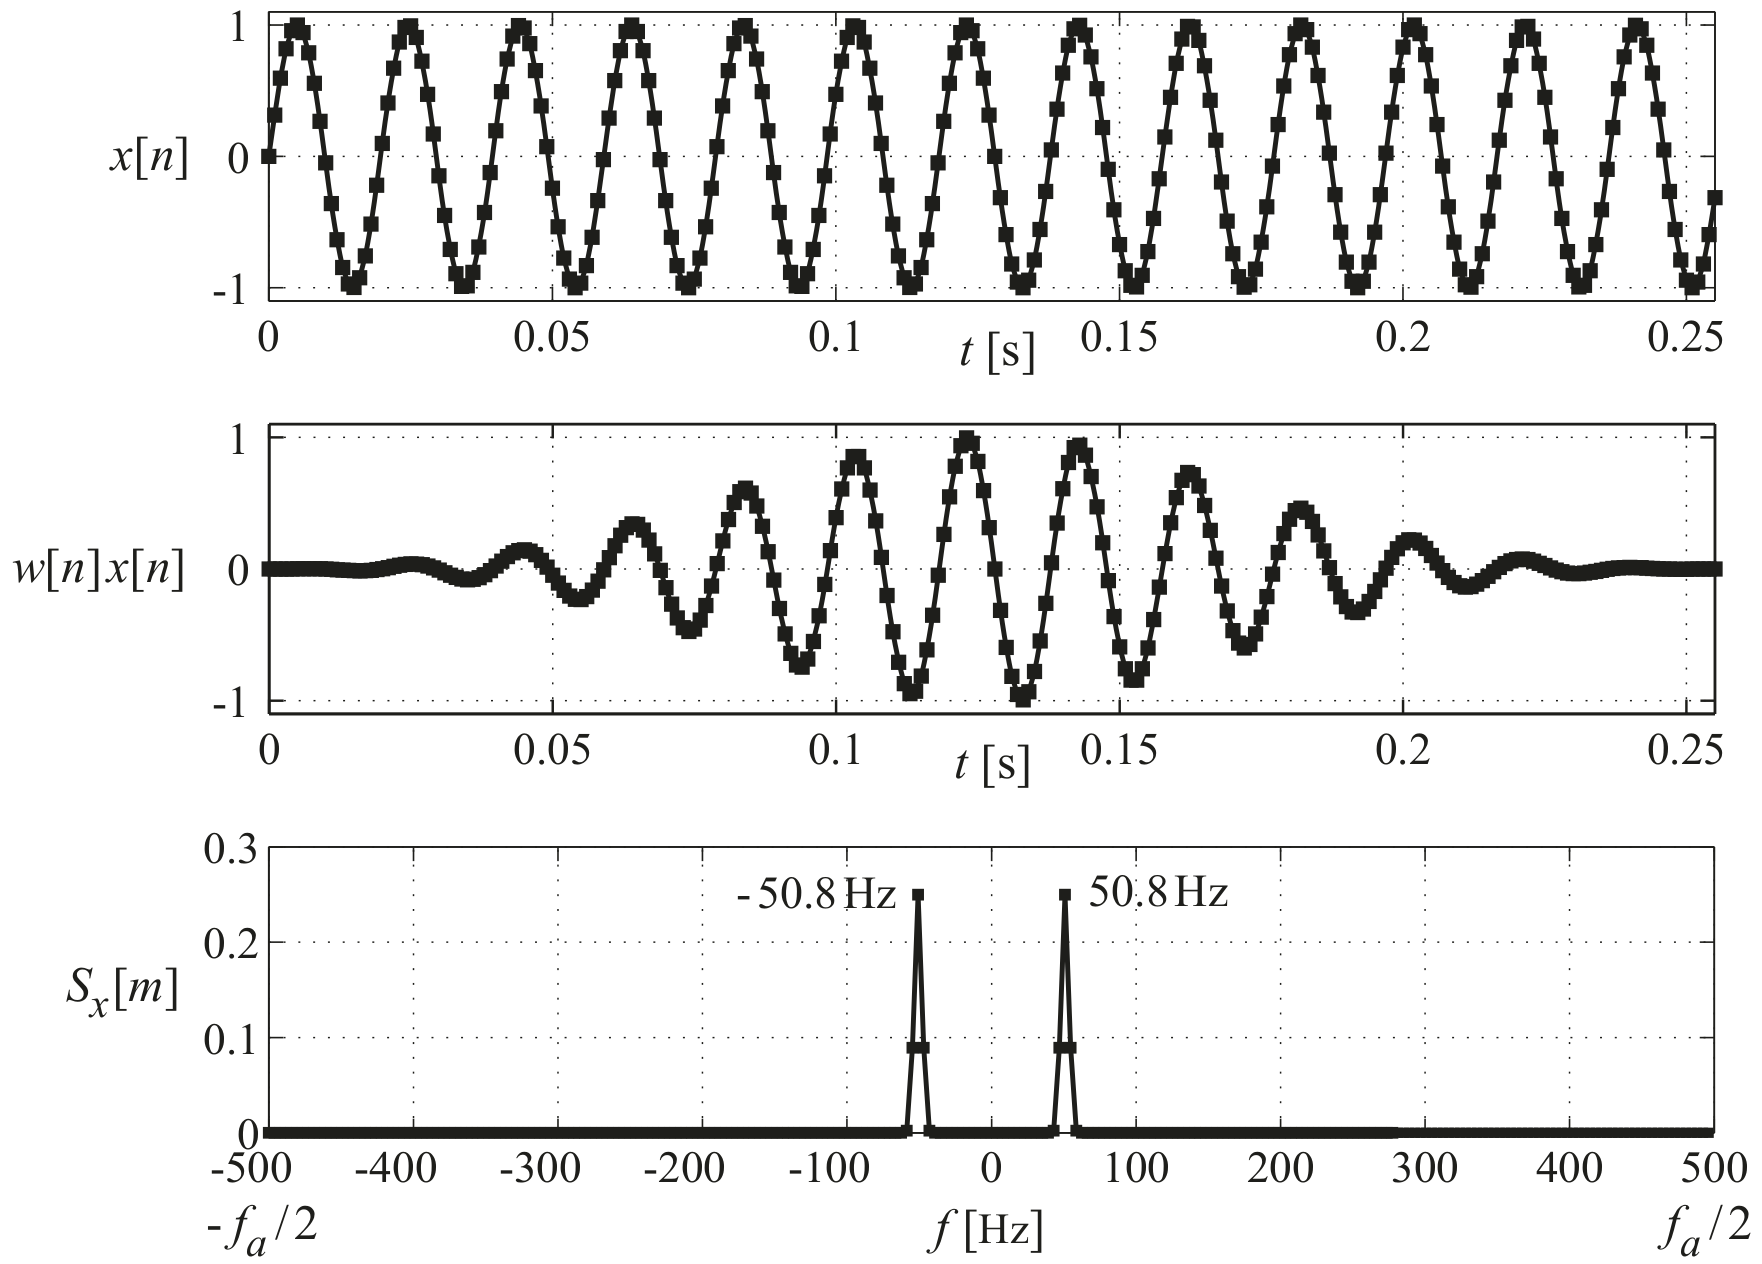
\includegraphics[width=\textwidth]{FFT.png}
	\caption[Zeitsignal, gefenstertes Zeitsignal und Spektrum eines diskreten Sinus-Signals]{Zeitsignal, gefenstertes Zeitsignal und Spektrum eines diskreten Sinus-Signals. Quelle: \cite[Heuberger, e. a., S. 16]{Heuberger:2017}} 
	\label{fft}
\end{figure}




\section{Basisbandübertragung und Trägersignale}
Die Übertragung von Signalen kann über verschiedene Medien erfolgen, etwa über metallische Leiter, Lichtwellenleiter oder über Funkstrecken. Eine Übertragung im sogenannten Basisband ist jedoch nur mit metallischen Leitern möglich \cite[vgl. Read, S. 149]{Read:2004}. Diese haben den Vorteil, dass ein Signal zur Übertragung den gesamten Frequenzbereich uneingeschränkt nutzen kann. Dies bedeutet, dass das volle Spektrum des Signals in den Übertragungskanal (z. B. Telefonleitung, LAN Kabel) eingespeist werden kann. Eine Verschiebung von den Frequenzen informationstragender Signale ist also nicht notwendig \cite[vgl. Werner, S. 158]{Werner:2006}. Ist das der Fall, so spricht man von einer Basisbandübertragung.\newline


\subsection{Modulationsverfahren}
Signale, die mit einer Funkübertragungstechnik gesendet werden, müssen vor der Übertragung jedoch an Frequenz und Bandbreite des entsprechenden Kanals angepasst werden \cite[vgl. Read, S. 24]{Read:2004}. 
Das hat unter anderem damit zu tun, dass für verschiedene Anwendungen spezielle Bereiche im Frequenzspektrum reserviert sind, siehe Abschnitt \ref{section-frequenzbereiche}.
Des weiteren ist es zum Senden und Empfangen von Signalen vorteilhaft, wenn die Größe der Antenne in etwa der halben Wellenlänge des Signals entspricht \cite[vgl. Kark, S. 4]{Kark:2017}.
Bei der Übertragung von Sprachsignalen, welche (bei Männern) durchschnittlich bei etwa 120 Hz liegen, wäre zum Senden eine Antenne der Größe 1.250 km ideal:
\[ \frac{\lambda}{2} = \frac{c}{2f} = \frac{3*10^8 \text{ m/s}}{2*120 \text{ Hz}} = 1.250.000 \text{ m}\]

Da eine Antenne dieser Größe utopisch ist, können die zu übertragenden Informationen einfach auf höhere Frequenzen (mit entsprechend kleineren Wellenlängen) verschoben werden. Hierbei spricht man von \textit{Modulation}.
Die informationstragenden Signale werden dann bevorzugt einer elektromagnetischen, sinusförmigen Welle über die Amplitude, der Phase und/oder der Frequenz aufgeprägt \cite[vgl. Werner, S. 242f]{Werner:2017}. 

Bei der Modulation wird der Frequenzbereich des Basisbandes, also des zu modulierenden Signals, in einen anderen Frequenzbereich transformiert \cite[vgl. Plaßmann, S. 1204]{Plassmann:2016}.

\subsection{AM-Modulation}
Das Trägersignal, welchem die Informationen des Basisbandsignals aufgeprägt werden sollen, besitzt folgende allgemeine Form:
\[ x_{HF} (t) = a \cos(\omega_0t + \varphi) \text{ , wobei }\omega_0 = 2\pi f_0 \]

\(f_0\) ist die entsprechende Trägerfrequenz; Die Amplitude \(a\) und die Phase \(\varphi\) stehen für eine Modulation zur Verfügung \cite[vgl. Heuberger, e. a., S. 39]{Heuberger:2017}.

Die \ac{AM}, welche etwa bei AM-Rundfunk Verwendung findet, moduliert lediglich die Amplitude des Trägers. Bei der Amplitudenumtastung (engl. \ac{ASK}) eines digitalen Signals wird den zwei Stellungen von \(u_M\) je eine andere Amplitude \(u_{ASK}\) zugeordnet:

\begin{figure}[ht]
	\centering
	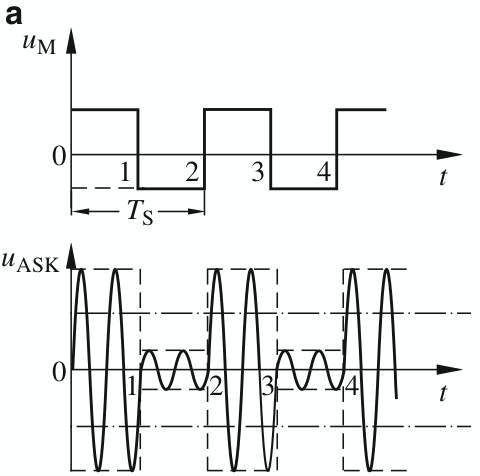
\includegraphics[width=0.4\textwidth]{ask-modulation.png}
	\caption[Amplitudenumtastung eines Digitalsignals]{Amplitudenumtastung eines Digitalsignals. Quelle: \cite[Plaßmann, S. 1218]{Plassmann:2016}} 
	\label{ask}
\end{figure}



\subsection{FM-Modulation}
Bei der FM Modulation wird die Amplitude des Signals konstant gehalten und stattdessen die Frequenz moduliert:
\[ x_{HF}(t) = a \cos (\omega_0 t + \varphi)t  \text{  mit } \varphi(t) = \int_{- \infty}^{t} \omega(t_1) dt_1\] 
Dafür können bei digitalen Signalen einfach zwei Frequenzen \(f_1\) und \(f_2\) verwendet werden:
\begin{figure}[ht]
	\centering
	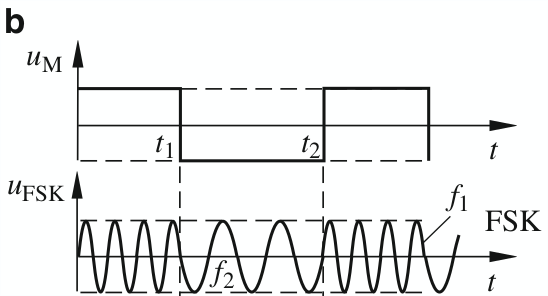
\includegraphics[width=0.45\textwidth]{fsk-modulation.png}
	\caption[Frequenz- und Phasenumtastung eines Digitalsignals]{Frequenz- und Phasenumtastung eines Digitalsignals. Quelle: \cite[Plaßmann, S. 1218]{Plassmann:2016}} 
	\label{fsk}
\end{figure}



\subsection{I/Q-Modulation}
\label{iq}
\ac{AM} und \ac{FM} lassen sich theoretisch kombinieren um die Übertragungskapazität zu steigern, jedoch wird das in der Praxis nicht getan, da AM und FM unterschiedliches Verhalten aufweisen und die beiden Kanäle somit nicht gleichwertig sind \cite[vgl. Heuberger, e. a., S. 40]{Heuberger:2017}. Um das aber zu erreichen, wird das Additionstheorem 
\[ \cos (\alpha + \beta) = \cos \alpha \cos \beta - \sin \alpha \sin \beta\] 
auf die Kombination von AM und FM angewandt:
\begin{align*}
	x_{HF}(t) &= a(t) \cos (\omega_0 t + \varphi(t)) \\
			  &= \underbrace{a(t) \cos \varphi(t)}_{i(t)} \cos \omega_0(t) - \underbrace{a(t) \sin \varphi(t)}_{q(t)} \sin \omega_0t
\end{align*}

Dabei wird \(i(t) \)  als das \textit{Inphase-Signal} und \(q(t)\) als \textit{Quadratur-Signal} bezeichnet.
Da die Phase $\varphi(t)$ als Winkel betrachtet und zusammen mit der Amplitude $a(t)$ einen Vektor in der komplexen Zahlenebene ergibt, kann dieser mit Polarkoordinaten repräsentiert werden.
$i(t)$ und $q(t)$ werden als kartesische Koordinaten aufgefasst.
Das ermöglicht eine Umrechnung zwischen den beiden Darstellungen:
\[ i(t) = a(t) \cos \varphi(t),  \quad q(t) = a(t)\sin \varphi(t) \quad \text{und} \quad  a(t) = \sqrt{i^2 (t) + q^2(t)}\]
\[  \varphi (t) = \arctan \frac{q(t)}{i(t)}  
					\begin{cases} 
						0	 & \text{wenn } i(t) \geq 0 \\
						\pi  & \text{wenn } i(t) < 0
					\end{cases}
\]

Abb. \ref{ortskurven} stellt die Ortskurven der 3 Modulationsverfahren grafisch dar:
\begin{figure}[ht]
	\centering
	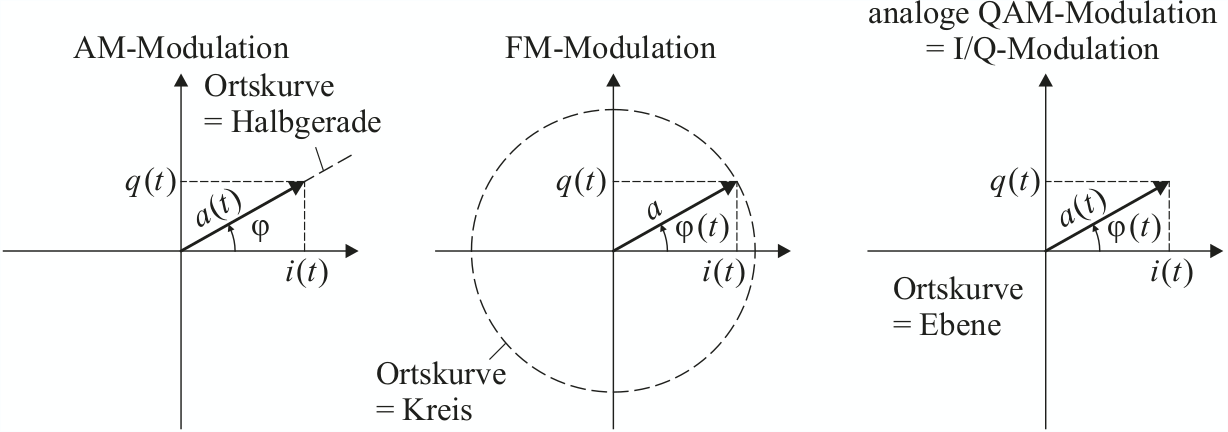
\includegraphics[width=\textwidth]{ortskurven.png}
	\caption[Ortskurven der Signale bei AM-, FM- und I/Q-Modulation]{Ortskurven der Signale bei AM-, FM- und I/Q-Modulation. Quelle: \cite[Heuberger, e. a., S. 141]{Heuberger:2017}} 
	\label{ortskurven}
\end{figure}


\newpage

Nach der eulerschen Formel ( \( e^{i\varphi} = cos \varphi + i \sin \varphi \) ) lassen sich die realen und imaginären Komponenten des Signals auch folgendermaßen darstellen:
\[ \underline{x} (t) = i(t) + jq(t) = a(t) e^{j \varphi(t)}\]

Es gilt zu beachten, dass in der Nachrichten- und Elektrotechnik häufig $j$ zur Darstellung von komplexen Zahlen benutzt wird, da $i$ meist bereits durch andere Größen, etwa der Stromstärke, oder wie hier - der \textit{realen} Inphase-Komponente belegt ist.
\newpage

\section{Software Defined Radio Systeme} 
\ac{SDR} Systeme sind digitale Datenübertragungssysteme, bei denen der Großteil der Signal- und Datenverarbeitung mittels Softwarekomponenten erfolgt \cite[Heuberger, e. a., S. 1]{Heuberger:2017}.
Besonders hervorzuheben ist bei \ac{SDR} Systemen, dass ihre Hardware größtenteils unabhängig nachrichtentechnischer Eigenschaften wie der Symbolrate und Modulationsart sind. \ac{SDR} Systeme können verschiedene Standards verwenden um entsprechende Übertragungsarten zu implementieren, da die Funktionalität durch Software, also hardwareunabhängig, realisiert wird \cite[Heuberger, e. a., S. 36]{Heuberger:2017}. \newline
Abbildung \ref{sdr-blockschaltbild} zeigt den Aufbau eines \ac{SDR} Systems als Blockschaltbild, in dem sowohl Sender und Empfänger als SDR realisiert sind.
Für jedes Element im Sender gibt es ein entsprechendes Element im Empfänger, welches die Senderoperationen rückgängig macht, um die ursprünglichen Daten rekonstruieren zu können.

Da sich diese Studienarbeit mit dem Empfangen und Auswerten von Signalen, aber nicht dem Senden befasst, wird im weiteren Verlauf des Dokumentes hauptsächlich die Seite des Empfängersystems und der Übertragungsstrecke betrachtet.

\begin{figure}[ht]
	\centering
	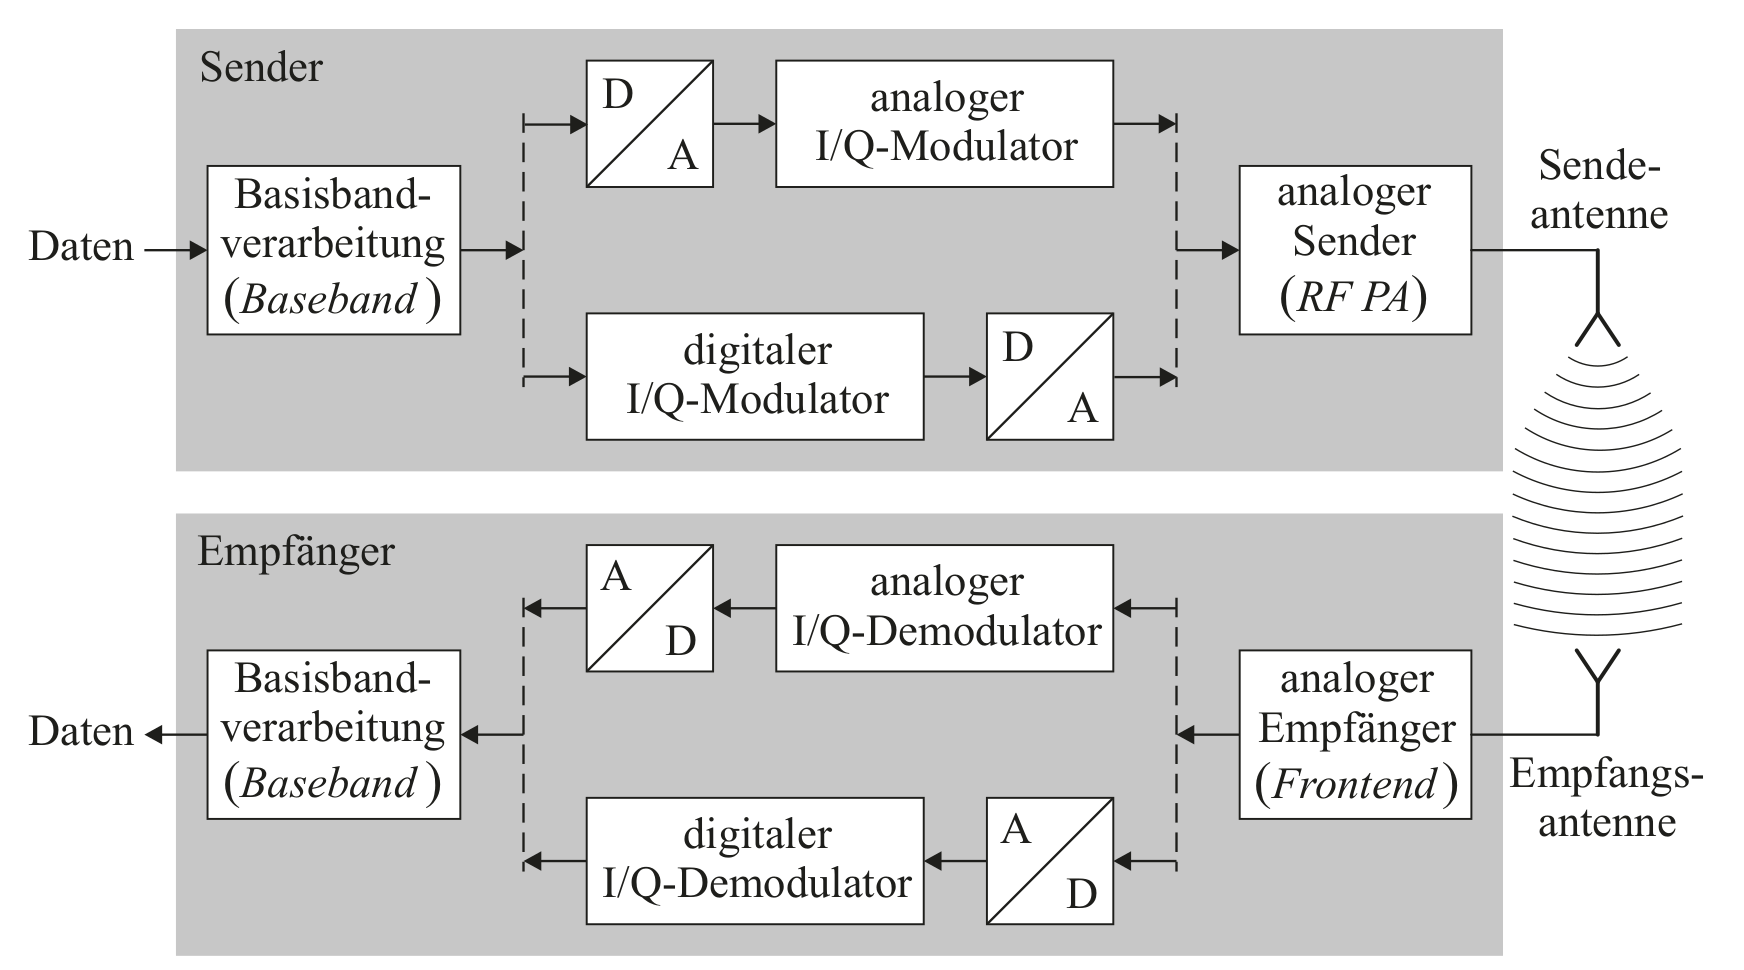
\includegraphics[width=0.9\textwidth]{sdr.png}
	\caption[Blockschaltbild eines SDR Systems]{Blockschaltbild eines SDR Systems. Quelle: \cite[Heuberger, e. a., S. 37]{Heuberger:2017}}
	\label{sdr-blockschaltbild}
\end{figure}

Abbildung \ref{nachrichtentechn-blockschaltbild} zeigt den Aufbau eines klassischen digitalen Übertragungssystems. Die Funktionsweise lässt sich wie folgt zusammenfassen:
\begin{description}
	\item [CRC Codierung] Um später die Integrität der digitalen Daten verifizieren zu können, werden sie mit einer \ac{CRC}-Codierung versehen.
	\item [Kanalcodierung] Digitale Daten werden bei der Übertragung über störbehaftete Kanäle üblicherweise mit Redundanzen versehen, um Übertragungsfehler abzuschwächen.
	\item [Scrambler] Ein sogenannter Scrambler (zu deutsch: \enquote{Verwürfler}) ist ein Pseudozufallszahlengenerator, der dafür sorgt, dass ein digitales Signal annähernd gleichmäßig verwürfelt wird. Dadurch sollen gleichbleibende Signalfolgen (etwa der Zustand \enquote{1}) über einen längeren Zeitraum vermieden werden. Dadurch wird die Leistung des Signals möglichst gleichmäßig über die genutzte Bandbreite verteilt \cite[vgl. Heuberger, e. a., S. 75]{Heuberger:2017}.
	\item [Symbol-Mapper] Aus binären Signalen erzeugt der Symbol-Mapper die entsprechenden Datensymbole, die Teil des zu verwendenden Alphabetes sind. 
	\item [Modulator] Das Signal wird abschließend einem Trägersignal aufgeprägt, damit es übertragen werden kann.
\end{description}

Anschließend erfolgen auf der Empfängerseite die entsprechenden inversen Operationen zu den aufgeführten Schritten. In einem Software Defined Radio System werden \textit{alle} diese Vorgänge durch Software in der Basisbandverarbeitung abgebildet \cite[vgl. Heuberger, e. a., S. 38]{Heuberger:2017}

\begin{figure}[ht]
	\centering
	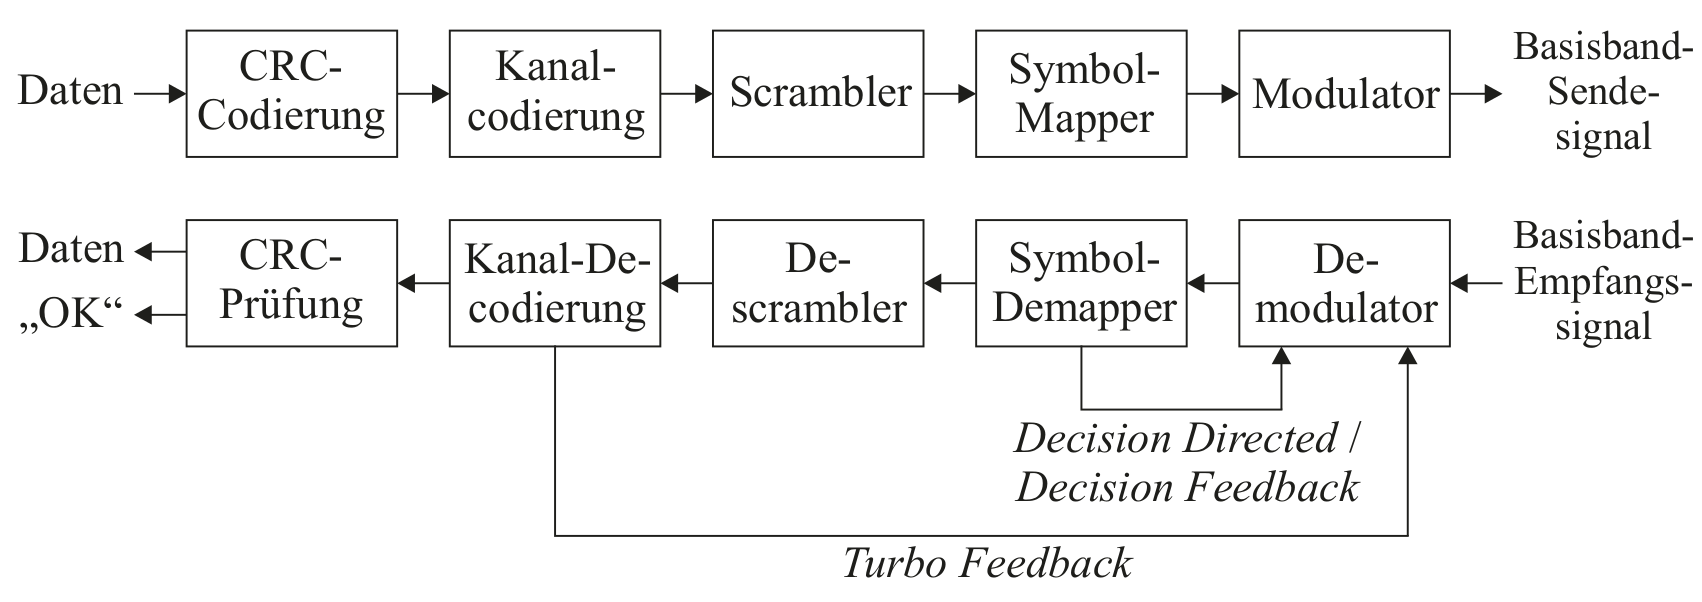
\includegraphics[width=\textwidth]{sdr-nachrichtentechn-blockschaltbild.png}
	\caption[Nachrichtentechnisches Blockschaltbild eines digitalen Übertragungssystems]{Nachrichtentechnisches Blockschaltbild eines digitalen Übertragungssystems. Quelle: \cite[Heuberger, e. a., S. 38]{Heuberger:2017}}
	\label{nachrichtentechn-blockschaltbild}
\end{figure}






